\documentclass[12pt, letterpaper]{article}

\title{My First Latex Document}
\author{Rana Universe\thanks{Mail Us AT: RanaUniverse321@gmail.com}}
\date{August 2025}


\usepackage{lipsum}

\usepackage{graphicx} %LaTeX package to import graphics
\graphicspath{{images/}} %configuring the graphicx package

% \renewcommand{\figurename}{Graph Image}
% To get Figure 1,2,3... i will use normal, if i want custom name i will uncomment this upper, which will say, Graphh Image 1, 2, 3 ...


\usepackage{pgffor} % For loops i will use this package so that i can use repetative work easily






\begin{document}

\maketitle






\begin{figure}[htbp]
\centering

\fbox{

\includegraphics[width=0.5\textwidth]{rana_universe_logo_round_black.png}
}

\caption{Rana Universe logo in black circle}

\label{fig:rana-universe-logo}

\end{figure}





\newpage


The mass-energy equivalence is described by the famous equation

\[E=mc^2\]

discovered in 1905 by Albert Einstein. 
In natural units ($c$ = 1), the formula expresses the identity

\begin{equation}
E=m
\end{equation}


% This is the variable type of things, i will use this below and use the value.
\newcommand{\titlevariable}{Let's Start Using the \textbf{`amsmath'}}


\noindent\rule{\linewidth}{5pt}
\begin{center}
\titlevariable \par
\end{center}
\noindent\rule{\linewidth}{5pt}


\begin{center}
\noindent\rule{\linewidth}{5pt} \\
% Let's Start Using the \textbf{`amsmath'} \par
\titlevariable \par
\noindent\rule{\linewidth}{5pt}
\end{center}




\newpage


The well known Pythagorean theorem \(x^2 + y^2 = z^2\) was 
proved to be invalid for other exponents. 
Meaning the next equation has no integer solutions:

\[ x^n + y^n = z^n \]


Here is a famous quote:

\begin{quote}
In physics, the mass-energy equivalence is stated 
by the equation \(E=mc^2\), discovered in 1905 by Albert Einstein.
\end{quote}

And now back to the main text.




\noindent Standard \LaTeX{} practice is to write inline math by enclosing it between \verb|\(...\)|:

\begin{quote}
In physics, the mass-energy equivalence is stated 
by the equation \(E=mc^2\), discovered in 1905 by Albert Einstein.
\end{quote}

\noindent Instead if writing (enclosing) inline math between \verb|\(...\)| you can use \texttt{\$...\$} to achieve the same result:

\begin{quote}
In physics, the mass-energy equivalence is stated 
by the equation $E=mc^2$, discovered in 1905 by Albert Einstein.
\end{quote}

\noindent Or, you can use \verb|\begin{math}...\end{math}|:

\begin{quote}
In physics, the mass-energy equivalence is stated 
by the equation \begin{math}E=mc^2\end{math}, discovered in 1905 by Albert Einstein.
\end{quote}








\newpage

The equation $a + b = c$ is simple.

\[ a^2 + b^2 = c^2\]


\begin{equation}
	a + b = c
\end{equation}

\begin{equation}
a^2 + b^2 = c^2
\end{equation}

\begin{equation}
	a^3 + b^3 = c^3
\end{equation}

\begin{equation}
a^4 + b^4 = c^4
\end{equation}

% This below will start from as usual sentence.
$
a + b,\quad a - b,\quad a \times b,\quad a \div b
$

% This below 2 things are same output, this are just for choice i will use.

\[
a + b,\quad a - b,\quad a \times b,\quad a \div b
\]


\[
a + b,\quad 
a - b,\quad 
a \times b,\quad 
a \div b
\]





\vspace{10\baselineskip}

I love this Upper Examples.



\newpage





\mbox{}


\newpage





\foreach \name in {Rana, Universe, RanaUniverse} {
    Hello, \textbf{\name!} \par
}


\vspace{5em}
\foreach \n in {1,...,9} {
    I am Rana Universe...\textbf{(\n)} \par
}

\vspace{3em}

\foreach \n in {1,...,9} {
    
    \noindent \textbf{\n.} I am Rana Universe... \par

    \textbf{\n.} I am Rana Universe... \par
}



\begin{figure}[ht]   % Start figure environment
    \centering   % Center the image

    % 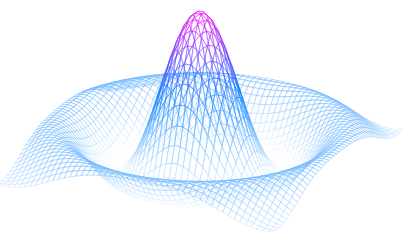
\includegraphics[width=.5\textwidth]{mesh.png}    

    % This below is for adding a black border
    \fbox{
        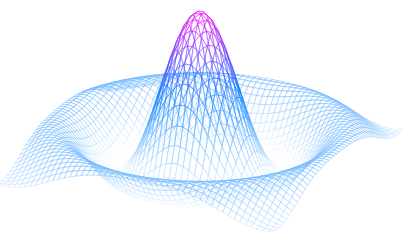
\includegraphics[width=0.5\textwidth]{mesh.png}
    }

    \caption{\textbf{A nice plot.}}   
    \label{fig:mesh1}   % Label: Internal name used to reference the figure, it should be unique
\end{figure}


As you can see in \textbf{Figure \ref{fig:mesh1}}, the function grows near the origin. This example is on page \pageref{fig:mesh1}.


As you can see in \textbf{\textit{Figure \ref{fig:mesh1}}}, the function grows near the origin. This example is on page \pageref{fig:mesh1}.



\begin{figure}[htbp]
	\centering
	
\includegraphics[width=0.5\textwidth]{linux_logo.png}
	\caption{\textbf{Linux Logo}}
	\label{fig:linuxlogo}
\end{figure}

Now in \textit{Figure \ref{fig:linuxlogo}}, you can see the famous Linux logo.
This is shown on page \pageref{fig:linuxlogo}.





\vspace{10em}

I am Rana Universe...

I am Rana Universe...

I am Rana Universe...

I am Rana Universe...

I am Rana Universe...

I am Rana Universe...

I am Rana Universe...

I am Rana Universe...

I am Rana Universe...

\vspace{3em}





\lipsum[1]

\lipsum[2]

\vspace{1em}

\lipsum[1]




% This line here is a comment. It will not be typeset in the document.
\end{document}



